%%%%%%%%%%%%%%%%%%%%%%%%%%%%%%%%%%%%%%%%%
% University/School Laboratory Report
% LaTeX Template
% Version 3.1 (25/3/14)
%
% This template has been downloaded from:
% http://www.LaTeXTemplates.com
%
% Original author:
% Linux and Unix Users Group at Virginia Tech Wiki
% (https://vtluug.org/wiki/Example_LaTeX_chem_lab_report)
%
% License:
% CC BY-NC-SA 3.0 (http://creativecommons.org/licenses/by-nc-sa/3.0/)
%
%%%%%%%%%%%%%%%%%%%%%%%%%%%%%%%%%%%%%%%%%

%----------------------------------------------------------------------------------------
%	PACKAGES AND DOCUMENT CONFIGURATIONS
%----------------------------------------------------------------------------------------

\documentclass[12pt]{article}

\usepackage[version=3]{mhchem} % Package for chemical equation typesetting
\usepackage{ctex}
\usepackage{siunitx} % Provides the \SI{}{} and \si{} command for typesetting SI units
\usepackage{graphicx} % Required for the inclusion of images
\usepackage{natbib} % Required to change bibliography style to APA
\usepackage{amsmath} % Required for some math elements

\setlength\parindent{0pt} % Removes all indentation from paragraphs

\renewcommand{\labelenumi}{\alph{enumi}.} % Make numbering in the enumerate environment by letter rather than number (e.g. section 6)

%\usepackage{times} % Uncomment to use the Times New Roman font

%----------------------------------------------------------------------------------------
%	DOCUMENT INFORMATION
%----------------------------------------------------------------------------------------

\title{性能优化分析实验报告} % Title
\author{劳马东 \textsc{16337113}\\数据科学与计算机学院\\计算机科学与技术(超算方向)} % Author name
\date{\today} % Date for the report
\begin{document}
\maketitle % Insert the title, author and date

% If you wish to include an abstract, uncomment the lines below
% \begin{abstract}
% Abstract text
% \end{abstract}

%----------------------------------------------------------------------------------------
%	SECTION 1
%----------------------------------------------------------------------------------------

\section{图像旋转}
\subsection{简单旋转}
当发生cache缺失时,数据会从高级存储层次拷贝到低级存储层次(如从L2 cache到L1 cache),拷贝的单位
是一条cache line(或者说一个块)而不是所访问的一个数据单位。cache line的典型大小时64B,在本例
中就是32个pixel的大小,L1 cache的大小为32K。图1中的代码是一个简单的二位数组循环,从L1数据cache利用率的角度来讲,
\begin{enumerate}
  \begin{item}
    对src数组的访问,空间局部性较好,每读32个pixel会导致一次L1级cache缺失(cache line的长度
    为64个字节),因此cache缺失次数为:
    \begin{equation}
      dim \times \frac{dim}{32} = \frac{dim^2}{32}
    \end{equation}
  \end{item}
  \begin{item}
    对dst数组的访问,空间局部性极差,假设dim大于L1级数据cache的行数,那么对dst的每一次写操作
    都会导致一次缺失,因此cache缺失次数为:
    \begin{equation}
      dim \times dim = dim^2
    \end{equation}
  \end{item}
\end{enumerate}
于是总的cache缺失次数为:
\begin{equation}
  \frac{dim^2}{32} + dim^2 = \frac{33dim^2}{32}
\end{equation}

\begin{figure}[h]
\begin{center}
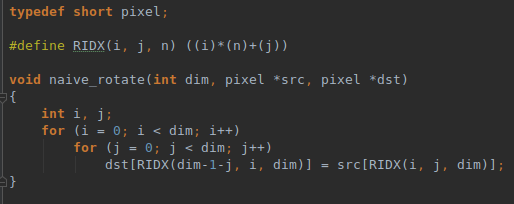
\includegraphics[width=\textwidth]{c0.png} % Include the image placeholder.png
\caption{简单旋转}
\end{center}
\end{figure}

\subsubsection{测试结果}
测试数组$dim=2048$,用$perf stat$指令记录L1数据cache的读取和缺失次数。如图2,总共读取59148201次,
发生5173774次cache缺失,缺失率为8.75\%。
\begin{figure}[h]
\begin{center}
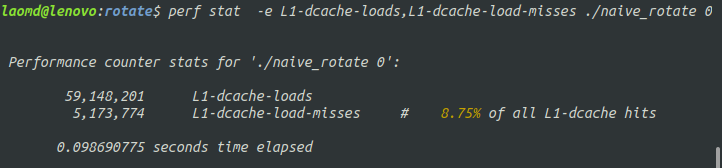
\includegraphics[width=\textwidth]{p0.png} % Include the image placeholder.png
\caption{简单旋转结果}
\end{center}
\end{figure}

\newpage
\subsection{第一次尝试:$4 \times 4$分块}
在图1中,对dst的写操作一次仅仅只是利用了一条cache line的一个数据单位。为了增加写操作的空间局部性,
提高cache line的利用率,可采用分块的方法。图3采用了$4 \times 4$分块,读操作的cache缺失图一相同,
而写操作的cache缺失数目减少,一次连续利用了一条cache line的4个数据单位,即每写4次发生一次缺失,
因此,写操作的cache缺失数目为:
\begin{equation}
  dim \times \frac{dim}{4} = \frac{dim^2}{4}
\end{equation}
总的cache缺失数目为:
\begin{equation}
  \frac{dim^2}{32} + \frac{dim^2}{4} = \frac{9dim^2}{32}
\end{equation}

\begin{figure}[h]
\begin{center}
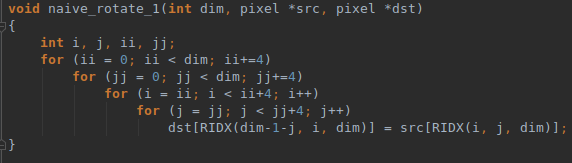
\includegraphics[width=\textwidth]{c1.png} % Include the image placeholder.png
\caption{$4 \times 4$分块}
\end{center}
\end{figure}

\subsubsection{测试结果}
如图4,$4 \times 4$分块的cache缺失的次数明显比不分块的小很多,是其
$\frac{1547961}{5173774}\approx \frac{1}{3.34}\approx \frac{\frac{9dim^2}{32}}{\frac{33dim^2}{32}}$
\begin{figure}[h]
\begin{center}
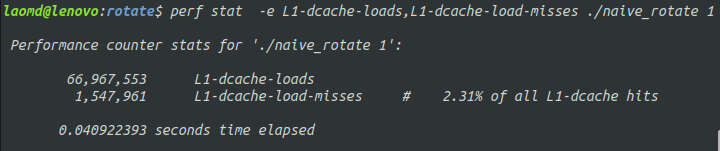
\includegraphics[width=\textwidth]{p1.png} % Include the image placeholder.png
\caption{$4 \times 4$分块结果}
\end{center}
\end{figure}

\newpage
\subsection{第二次尝试:循环展开}
一条cache line最多可以存储32个pixel,因此采用$32 \times 32$分块对于写操做的cache利用率是最好的,
此时写操作的cache缺失数目为:
\begin{equation}
  \frac{dim^2}{32}
\end{equation}
故总的cache缺失数目为:
\begin{equation}
  \frac{dim^2}{32} + \frac{dim^2}{32} = \frac{dim^2}{16}
\end{equation}
此外,循环展开可以降低循环开销,为具有多个功能单元的处理器提供指令级并行。如图6是该方案的代码。

\subsubsection{测试结果}
如图5:
\begin{figure}[h]
\begin{center}
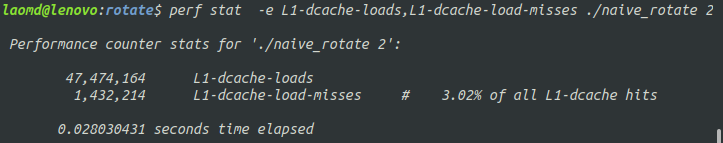
\includegraphics[width=\textwidth]{p2.png} % Include the image placeholder.png
\caption{$32 \times 32$分块,$4 \times 4$路循环展开结果}
\end{center}
\end{figure}

\begin{figure}[h]
\begin{center}
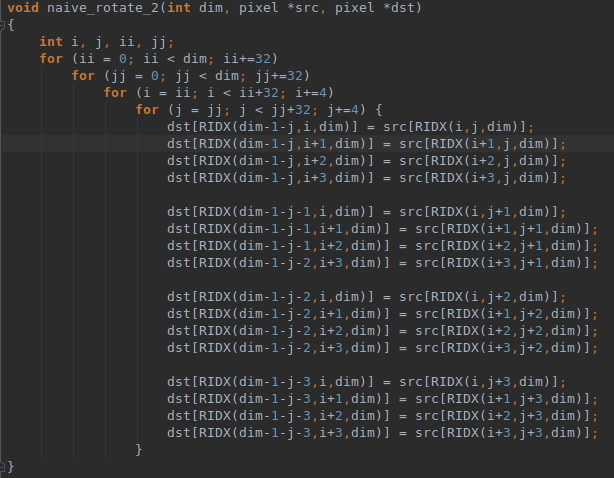
\includegraphics[width=\textwidth]{c2.png} % Include the image placeholder.png
\caption{$32 \times 32$分块,$4 \times 4$路循环展开}
\end{center}
\end{figure}

\newpage
\subsection{第三次尝试:采用不同的巡回路线}
第一次访问出现cache缺失的数据时,其对应的cache line被拷贝到cache,之后对该cache line其余
数据的访问都能命中。因此,对cache line元素的访问顺序不会影响cache缺失数,
即采用不同巡回路线的cache缺失数与第二次尝试相同。

\begin{figure}[h]
\begin{center}
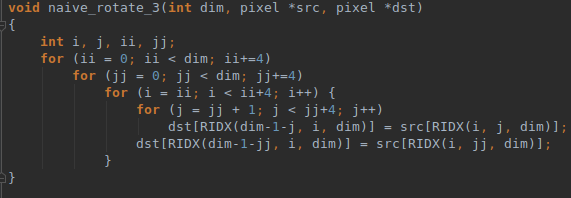
\includegraphics[width=\textwidth]{c3.png} % Include the image placeholder.png
\caption{$4 \times 4$分块,不同巡回路线}
\end{center}
\end{figure}

\subsubsection{测试结果}
\begin{figure}[h]
\begin{center}
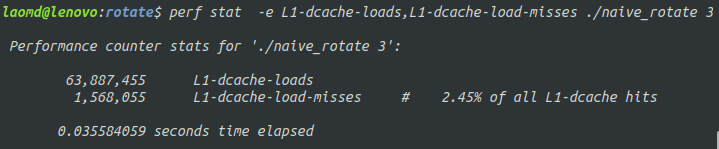
\includegraphics[width=\textwidth]{p3.png} % Include the image placeholder.png
\caption{$4 \times 4$分块,不同巡回路线结果}
\end{center}
\end{figure}

\newpage
\subsection{最后的尝试}
分块的两个维度的大小分别影响这src和dst数组。第一维的大小决定连续访问src数组的多少个元素以及访问
dst数组连续元素的频率,第二维同理,因此需要一个折中。显然,连续访问dst数组的元素是有好处的,这样
可以减少cache line写回的次数,也就节省了时间。
\par 对于图9中的方案,采用$32 \times 1$分块,读操作在访问了一列的32个元素后重新回到第一行,即
访问同一条cache line的频率是$\frac{1}{32}$,能及时地利用被拷贝的cache line,
而写操作在dst数组中访问了一行连续的32个元素,这是最优的;再将对32个元素的访问展开,就能并行地利用多个功能单元,增加指令级并行。

\begin{figure}[h]
\begin{center}
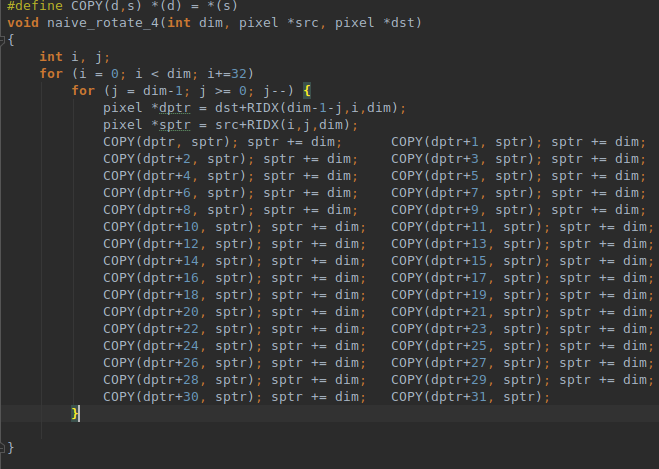
\includegraphics[width=\textwidth]{c4.png} % Include the image placeholder.png
\caption{$32 \times 1$分块,32路循环展开}
\end{center}
\end{figure}

\subsubsection{测试结果}
\begin{figure}[h]
\begin{center}
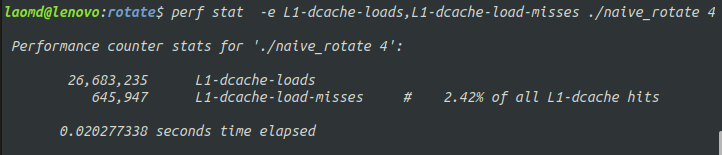
\includegraphics[width=\textwidth]{p4.png} % Include the image placeholder.png
\caption{$32 \times 1$分块,32路循环展开结果}
\end{center}
\end{figure}

\end{document}
